% !TEX encoding = UTF-8
% !TEX TS-program = pdflatex
% !TEX root = ../tesi.tex

%**************************************************************
\chapter{Progetto di stage}
\label{cap:progetto-di-stage}
%**************************************************************


%**************************************************************
\section{Lo stage per San Marco Group}

Il concetto di stage formativo è molto importante per l'azienda San Marco Group. 
In primo luogo, viene considerata la sperimentazione di nuove tecnologie ed il loro confronto con quelle utilizzate quotidianamente. Per poterlo fare attualmente il personale presente dovrebbe smettere di svolgere le proprie attività, per questo motivo uno stagista universitario diventa una risorsa indispensabile, permettendo quindi all'azienda di sperimentare senza che vengano bloccate le normali mansioni.
Ci sono diverse realtà all'interno dell'azienda che possono considerarsi formative per uno studente e che attuano costantemente questa collaborazione:
\begin{itemize}
	\item \textbf{l'ufficio Risorse Umane}, dove studenti del settore giuridico o umanistico possono crescere trovandosi in un'azienda con un grande gruppo eterogeneo di membri; 
	\item \textbf{l'ufficio Marketing}, molto sviluppato nell'azienda che dà spazio a figure che hanno intrapreso studi in ambito grafico o orientati alle comunicazioni e al marketing web;
	\item \textbf{il laboratorio di Ricerca e Sviluppo}, la sezione, presente nella sede di Marcon, affianca studenti del settore chimico ad un gruppo di chimici \textit{senior} che svolge attività di studio e ricerca su pitture decorative e decorativi per pavimenti, prodotti per le facciate, rivestimenti e sistemi termoisolanti; 
	\item \textbf{i Back office}, che comprendono l'ufficio Acquisti e l'ufficio Commerciale, dove studenti nel settore economico e commerciale hanno modo di confrontarsi con una realtà molto sviluppata e affermata nel territorio.
\end{itemize}
In secondo luogo, l'instaurazione del rapporto con l'Università di Padova è dato dalla possibilità di inserimento nell'azienda di risorse derivanti dal mondo accademico che, con una nuova prospettiva data dalle conoscenze apprese e messe in pratica nel corso di studio, possono portare idee creative e innovative, dalle quali può trarre beneficio anche il personale aziendale.

%**************************************************************
\section{Contesto attuale}

Attualmente l'azienda è nel vivo di un progetto di cambio gestionale, motivato principalmente da:
\begin{itemize}
	\item la fine del supporto da parte di \textit{Microsoft}, sul gestionale attualmente adottato (\textit{Microsoft Dynamics Ax 2009}) fissato per il 12 ottobre 2021;
	\item insoddisfazione da parte della direzione sul prodotto.
\end{itemize}
Nonostante ci fosse la possibilità di continuare ad utilizzare la versione 2009 anche oltre alla fine del supporto, affidandosi ad un partner terzo per la manutenzione e le implementazioni dei vari adeguamenti necessari a soddisfare periodicamente le regole stabilite nel contesto fiscale, tale decisione è stata ritenuta troppo rischiosa perché in caso di inadempienze del partner scelto, ci sarebbero potute essere conseguenze importanti per l'azienda, come ad esempio l'impossibilità di adempiere agli obblighi fiscali.
Si è deciso quindi di effettuare l'analisi di tutti i processi aziendali così da individuarne le criticità: in questo modo il cambio di software non avrebbe solamente soddisfatto le necessità ma anche portato un miglioramento. In seguito all'analisi supportata da un'azienda di consulenza, è iniziata la \textit{software selection}.

\vspace{10pt}
\begin{figure}[htbp]
	\begin{center}
		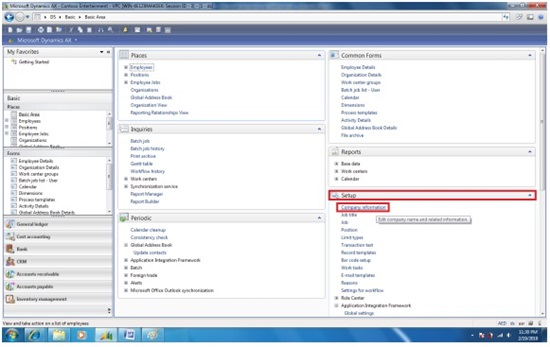
\includegraphics[height=8cm]{ax-2009}
		\caption{Interfaccia utente \textit{Microsoft Dynamics Ax 2009}. \newline \textbf{Fonte: }\url{https://community.dynamics.com/}}
	\end{center}
\end{figure}
\vspace{10pt}

Tra i vari software gestionali presenti sul mercato, è stato preso in considerazione \textit{Microsoft Dynamics 365}. La nuova versione dell'\textit{ERP} di \textit{Microsoft} differisce in maniera sostanziale da quella attualmente utilizzata, principalmente per quanto riguarda:
\begin{itemize}
	\item la re-ingegnerizzazione della base di dati, che richiederebbe una reimpostazione radicale della base di dati attuale;
	\item la dismissione del modello di sviluppo a \textit{layer}, che consiste nell'utilizzo di una gerarchia di livelli nei quali vengono implementati i metodi degli elementi applicativi presenti nel gestionale. Quando viene eseguito un metodo di un qualsiasi elemento applicativo, il sistema parte dal \textit{layer} più esterno per verificare ed eseguire, se disponibile, un'implementazione del metodo per quell'elemento, altrimenti si sposta sul \textit{layer} più interno per ripetere l'operazione fino ad arrivare al \textit{layer} di sistema.In questo modo è possibile personalizzare facilmente le varie funzionalità presenti, attività che con la nuova versione richiederebbero un processo più impegnativo.
\end{itemize}
L'adozione di \textit{Microsoft Dynamics 365} sarebbe stata troppo impegnativa dal punto di vista tecnico sia nel breve che nel lungo termine, per questo motivo è stato scartato.
Alla fine della valutazione la scelta è ricaduta su Sage X3, per la sua adattabilità e perché rispecchia maggiormente le necessità aziendali; è perciò iniziata la fase di implementazione del nuovo software attraverso:

\begin{itemize}
	\item sviluppi per adeguamento delle funzionalità del nuovo gestionale agli standard aziendali;
	\item migrazione dei dati;
	\item formazione degli utenti finali.
\end{itemize}


\vspace{10pt}
\begin{figure}[htbp]
	\begin{center}
		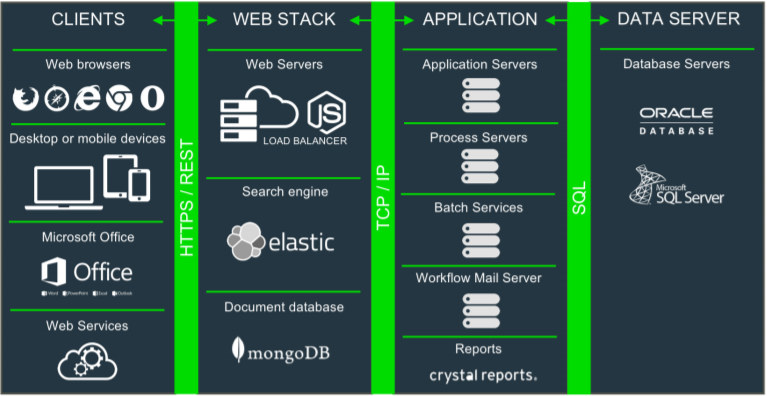
\includegraphics[height=7cm]{sage-x3}
		\caption{Architettura di sistema di Sage X3. \newline \textbf{Fonte: }\url{https://partnerportal.sagex3.com/}}
	\end{center}
\end{figure}
\vspace{30pt}


%**************************************************************
\section{Proposta di stage}

Lo scopo dello stage consisteva nello sviluppo software di un sistema di gestione di offerte di fornitura, dedicate a beni materiali e servizi. Dopo l'analisi del processo, lo studente doveva sviluppare un'applicazione web che permettesse agli utenti interni la gestione delle richieste e ai fornitori designati di rispondere con delle proposte di offerta.
L'applicazione da sviluppare doveva avere le seguenti caratteristiche:
\begin{itemize}
	\item interfacciarsi con il database del gestionale tramite \textit{web services};
	\item la sezione destinata alle richieste di servizio di trasporto doveva rispettare il layout del modulo cartaceo utilizzato;
\end{itemize}
Doveva essere prodotto un \textit{report} con il dettaglio della richiesta e in base al tempo disponibile, lo studente doveva riuscire a fornire delle statistiche sulla base dei dati utilizzati, utili all'analisi di \textit{business intelligence}, in ottica di miglioramento del processo aziendale.


\subsection{Prodotti attesi}
L'attività di stage doveva prevedere la produzione dei seguenti oggetti, documenti e software:
\begin{itemize}
	\item relazione sul processo aziendale coinvolto;
	\item relazione sulla progettazione architetturale;
	\item codice sorgente dell'applicazione web;
	\item manuale e documentazione riguardante la struttura dell'applicazione web per
	manutenzione ed eventuali integrazioni;
	\item report di dettaglio dell'offerta;
	\item report con statistiche utili all'analisi di \textit{business intelligence}.
\end{itemize}


\subsection{Priorità e obiettivi dello stage}
Per identificare gli obiettivi ed il loro livello di priorità, si associa a ciascuno di essi un codice con il formato sottostante:
\\
\begin{center}
	\textit{<obiettivo.[sotto-obiettivo]-tipologia>. }
\end{center}
Il significato del codice è il seguente:
\begin{itemize}
\item \textbf{obiettivo}, indica il numero univoco dell'obiettivo;
\item \textbf{sotto-obiettivo}, è il numero univoco del sotto-obiettivo, ed è opzionale, essendo riportato solo nel caso in cui l'obiettivo sia suddiviso in sotto-obiettivi;
\item \textbf{tipologia}, indica il livello di priorità assegnato all'obiettivo.
\end{itemize}
La tipologia determina l'importanza di realizzare tale obiettivo, ed è scelta tra le seguenti:
\begin{itemize}
	\item \textbf{OB}, indica un obiettivo obbligatorio, il cui raggiungimento è necessario;
	\item \textbf{DE}, indica un obiettivo desiderabile, il cui raggiungimento è importante e dal riconoscibile valore aggiunto, ma non necessario.
\end{itemize}

\begin{table}
\caption{Tabella che riassume gli obiettivi dello stage.}
\label{tab:requisiti-stage}
\begin{tabularx}{\textwidth}{lXl}
\hline\hline
\textbf{Obiettivo} & \textbf{Descrizione}\\
\hline
1-OB & Comprensione del problema\\
\hline
2-OB & Comprensione delle tecnologie di \textit{backend}\\
\hline
2.1-OB & Comprensione di \textit{Sage X3}\\
\hline
2.2-OB & Comprensione del database \textit{SQL Server}\\
\hline
2.3-OB & Comprensione della tecnologia dei \textit{web services}\\
\hline
3-OB & Comprensione delle tecnologie di \textit{frontend}\\
\hline
3.1-OB & Comprensione di \textit{Javascript}\\
\hline
3.2-OB & Comprensione di \textit{JQuery}\\
\hline
4-OB & Sviluppo dell'interfaccia \textit{web}\\
\hline
5-OB & Sviluppo del report per tracciamento caratteristiche offerta
\\
\hline
6-OB & Validazione del prodotto\\
\hline
7-DE & Sviluppo del report per statistiche miglioramento \textit{BI}\\
\hline
\end{tabularx}
\end{table}

\subsection{Vincoli}
\subsubsection{Vincoli temporali e organizzativi}
Il progetto di stage ha avuto una durata di 320 ore, distribuite nell'arco di tre mesi, con settimane lavorative di 25 ore ciascuna.
In accordo con il relatore e il tutor aziendale, lo stage è stato svolto prevalentemente in modalità \textit{smart working}.
Per poter informare il mio relatore  dei progressi, è stato stabilito l'invio di un resoconto ogni 5 giorni lavorativi dello stato di avanzamento rispetto alle attese del piano di lavoro e ad eventuali deviazioni da esso.\\Invece, con il tutor aziendale, è stato previsto almeno un incontro a settimana in remoto o fisicamente in azienda per discutere del progresso e di eventuali cambiamenti da apportare al progetto.
\subsubsection{Vincoli tecnologici}
Lo sviluppo del progetto prevedeva alcuni vincoli imposti dall'azienda.
In primo luogo l'utilizzo della tecnologia \textit{SOAP}, \textit{Simple Object Access Protocol}, per i \textit{web services} che permettevano l'interfacciamento tra l'applicazione \textit{web} e il gestionale.
In secondo luogo, l'utilizzo dello strumento per la produzione di stampe di dati \textit{Crystal Reports} per produrre il report di dettaglio della richiesta d'offerta e il report con le statistiche utili all'analisi della \textit{business intelligence}.
%**************************************************************
\section{Analisi preventiva dei rischi}
Nella fase iniziale di analisi sono stati individuati alcuni possibili rischi in cui poter incorrere.\\
Si è quindi proceduto a elaborare delle possibili soluzioni per far loro fronte.
\\
\begin{risk}{Tecnologie e \textit{framework} sconosciuti}
	\riskdescription{Durante lo svolgimento dello stage è previsto l'utilizzo di tecnologie non ancora esplorate dallo studente}
	\risksolution{Nella fase di pianificazione iniziale è stato programmato un periodo di auto-formazione per le tecnologie e i \textit{framework} da utilizzare}	
\end{risk}
\begin{risk}{Incomprensioni sul processo aziendale}
	\riskdescription{A causa dei vari enti coinvolti nella fase di analisi e del gran numero di attività svolte attualmente extra sistema (utilizzo di moduli cartacei, contatti telefonici direttamente coi fornitori, ecc.), è possibile non venga ben delineato e compreso dallo studente il processo aziendale interessato}
	\risksolution{In accordo con il \textit{tutor} aziendale, sono stati individuati dei \textit{key users}, uno per ogni ufficio coinvolto, che si rendono disponibili ad offrire maggior dettaglio sulle fasi che interessano la loro attività}	
\end{risk}
\begin{risk}{Scelte non ottimali}
	\riskdescription{A causa dell'inesperienza dello studente è possibile non vengano comprese le attività da svolgere o vengano fatte scelte non adeguate alle aspettative.}
	\risksolution{Tutte le scelte progettuali fondamentali saranno discusse e supervisionate dal \textit{tutor} aziendale}	
\end{risk}

%**************************************************************
\section{Motivazione della scelta}

Una delle principali aspettative che mi hanno portato a scegliere questa proposta di stage
curriculare, era il contesto di inserimento: volevo capire come una grande azienda, il cui settore di impiego non è strettamente legato a quello informatico, si approccia alle nuove tecnologie e si appoggia all'informatica per il suo business.
Riuscire ad avere una visione d'insieme per capire quali attività vengono svolte per supportare un'azienda, non solo del contesto dello sviluppo software ma anche nell'ausilio di altri processi.\\ Inoltre, essendo in pieno sviluppo un progetto di cambio gestionale, ho ritenuto fosse un'opportunità ad alto contenuto formativo, sia per le tecnologie utilizzate a me ancora sconosciute, sia per la possibilità di interfacciarmi e collaborare direttamente con figure professionali interne ed esterne all'azienda impegnate nel progetto.\\
Mi interessava il fatto di potermi rapportare direttamente con gli utenti finali del prodotto, in modo da poter comprendere meglio le problematiche che si possono incontrare in fase di analisi e riuscire ad applicare i concetti studiati nel corso di Ingegneria del Software.
Inoltre, a conclusione dello stage mi attirava la possibilità di continuare a seguire le attività successive allo sviluppo del prodotto, come la formazione degli utenti, e vedere i risultati del mio lavoro nel lungo termine.
